\documentclass[9pt,twocolumn,twoside]{gsajnl}
\newcommand{\sme}[1]{\textcolor{red}{\bf #1}}
\newcommand{\yang}[1]{\textcolor{cyan}{\emph{\bf  #1}} }
\graphicspath{{Figure_Table/}} \newcommand{\beginsupplement}{        \setcounter{table}{0}
        \renewcommand{\thetable}{S\arabic{table}}        \setcounter{figure}{0}
        \renewcommand{\thefigure}{S\arabic{figure}}     }
\articletype{inv} 
\newcommand{\X}{\textcolor{red}{\bf X\,}}
\newcommand{\citex}{\textcolor{red}{\bf (CITE)\,}}
\newcommand{\jri}[1]{\textcolor{red}{ \emph{ #1}} }

\title{Incorporation of evolutionary constraint improves genomic prediction of inbred and hybrid phenotype} 
\author[$\ast$, 1, 2]{Jinliang Yang} \author[$\ast$, 2, 3]{Sofiane Mezmouk} \author[$\S$]{Andy Baumgarten} \author[$\dagger$]{Edward S. Buckler} \author[$\ddagger$]{Katherine E. Guill} \author[$\ddagger$, $\ast\ast$]{Michael D. McMullen} \author[$\S\S$]{Rita H. Mumm} \author[$\ast$, $\dagger\dagger$, 1]{Jeffrey Ross-Ibarra} 
\affil[$\ast$]{Department of Plant Sciences, University of California, Davis, CA 95616, USA}
\affil[$\S$]{DuPont Pioneer, Johnston, IA 50131, USA} \affil[$\dagger$]{US Department of Agriculture, Agricultural Research Service, Ithaca, NY 14853, USA} \affil[$\ddagger$]{US Department of Agriculture, Agricultural Research Service, Columbia, MO 65211, USA} \affil[$\ast\ast$]{Division of Plant Sciences, University of Missouri, Columbia, MO 65211, USA} \affil[$\S\S$]{Department of Crop Sciences, University of Illinois at Urbana-Champaign, Urbana, IL 61801, USA} \affil[$\dagger\dagger$]{Center for Population Biology and Genome Center, University of California, Davis, CA 95616, USA} 
\keywords{heterosis; deleterious; genomic selection; diallel; GERP; maize}

\runningtitle{Genomic Selection Using GERP score} 
\correspondingauthor{Jeffrey Ross-Ibarra}

\begin{abstract}
Complementation of deleterious alleles has long been proposed as a major contributor to the hybrid vigor observed in offspring of inbred parents.  We test this hypothesis using evolutionary measures of sequence conservation to ask whether incorporating information about putatively deleterious alleles can inform genomic selection (GS) models and improve phenotypic prediction. We measured a number of agronomic traits in both the inbred parents and hybrids of an elite maize partial diallel population.  We resequenced the parents of the population, using genomic evolutionary rate profiling (GERP) to identify constrained sites across more than 86 Mb of the genome.   We identifed haplotype blocks using an identity-by-decent analysis and scored these blocks on the basis of segregating putatively deleterious variants.  Incorporating sequence conservation improves prediction accuracies in a five-fold cross-validation experiment for several traits \emph{per se} as well as heterosis for those traits.  These results provide strong empirical support for the simple complementation model of heterosis, and demonstrates the utility of incorporatin functional annotation and its potential usage in phenotypic prediction and plant breeding.  \end{abstract}

\setboolean{displaycopyright}{true}
\RequirePackage[normalem]{ulem} \RequirePackage{color}\definecolor{RED}{rgb}{1,0,0}\definecolor{BLUE}{rgb}{0,0,1} \providecommand{\DIFadd}[1]{{\protect\color{blue}\uwave{#1}}} \providecommand{\DIFdel}[1]{{\protect\color{red}\sout{#1}}}                      \providecommand{\DIFaddbegin}{} \providecommand{\DIFaddend}{} \providecommand{\DIFdelbegin}{} \providecommand{\DIFdelend}{} \providecommand{\DIFaddFL}[1]{\DIFadd{#1}} \providecommand{\DIFdelFL}[1]{\DIFdel{#1}} \providecommand{\DIFaddbeginFL}{} \providecommand{\DIFaddendFL}{} \providecommand{\DIFdelbeginFL}{} \providecommand{\DIFdelendFL}{} 
\begin{document}

\maketitle
\thispagestyle{firststyle}
\marginmark
\firstpagefootnote
\DIFdelbegin \DIFdelend \DIFaddbegin \correspondingauthoraffiliation{Corresponding authors: Department of Plant Sciences, University of California, Davis, CA 95616, USA. Email: rossibarra@ucdavis.edu and jolyang@ucdavis.edu}
\DIFaddend \blfootnote{\textsuperscript{2}These authors contributed equally to this work}
\blfootnote{\textsuperscript{3}Current address: KWS SAAT AG, Grimsehlstr. 31, 37555 Einbeck, Germany}
\vspace{-11pt}


\DIFdelbegin 

\DIFdelend 
\lettrine[lines=2]{\color{color2}T}{}he phenomenon of heterosis or hybrid vigor has been observed across many species, from yeast \citep{Shapira2014} to plants \citep{shull1908composition} and vertebrates \citep{Gama2013}. 
A number of hypotheses have been put forth to explain the phenomenon, including gene dosage \citep{birchler2003search}, overdominance \citep{east1936heterosis, schwartz1973single, krieger2010flowering}\DIFdelbegin \DIFdel{or }\DIFdelend \DIFaddbegin \DIFadd{, }\DIFaddend pseudo-overdomiance \citep{graham1997characterization, McMullen2009}, and epistasis \citep{minvielle1987dominance, schnell1992multiplicative}. 
Complementation of recessive deleterious alleles, however, remains the simplest genetic explanation \citep{Charlesworth2009}, and \DIFaddbegin \DIFadd{one that }\DIFaddend is supported by considerable empirical evidences \citep{xiao1995dominance, frascaroli2007classical, huang2015genomic}.

\DIFdelbegin \DIFdel{Deleterious alleles were arisen from new mutations during meiosis. In maize, about 90 new mutations were generated per meiosis \mbox{\citep{Clark2005}
}, majority of which were deleterious according to empirical estimates \mbox{\citep{Joseph2004}
}. In a natural outcross population, the negative effects on fitness of these deleterious alleles make them subject to be selection against, which lead the deleterious alleles to be maintained in a low frequency \mbox{\citep{Eyre-Walker2007}
}. But the deleterious alleles could not be completely purged. 
}
\DIFdel{In maize, the total number of mildly deleterious mutations is substantial because of the exponential growth of population size after domestication. The modern breeding probably aims to remove these deleterious mutations and pyramiding beneficial alleles for agronomical purposes. In practice, the relatively homogeneous maizegermplasm pool was artificially divided into different heterotic groups \mbox{\citep{Heerwaarden2012}
}. 
It enabled the improvement of germplasm pools to be conducted in a parallel fashion, and therefore, facilitated the breeding efficiency. Using this hybrid breeding approach, }\DIFdelend \DIFaddbegin \DIFadd{One of }\DIFaddend the \DIFdelbegin \DIFdel{maize yield has been steadily improved since the early 20th century \mbox{\citep{duvick2001biotechnology}
}. However, removing deleterious mutations in low recombination regions or in tightly linked regions become less effective. Studies indicated that residual heterozygosity correlates negatively with recombination \mbox{\citep{Gore2009, McMullen2009}
}and the low recombination is effective over long period of time \mbox{\citep{Haddrill2007}
}. As a consequence, the deleterious alleles would be accumulated in the low recombination regions, such as the pericentromeric regions in maize, and the vigorous performance could be realized by combining two sets of non-deleterious or beneficial alleles in repulsion state, thus lead to pesudo-overdominance. A recent QTL study identified loci controlling for heterosis are enriched in centromeric regions \mbox{\citep{Lariepe2012}
}, which partly support this pesudo-overdominance hypothesis.
}\DIFdelend \DIFaddbegin \DIFadd{best studied examples of hybrid vigor is that of maize. 
Although the benefits of cross-fertilization or hybridization had been observed frequently in the past, it was not until the work of Shull, East, and others that it's significance for agriculture was well appreciated \citex.
Now, hybrid seed makes up the vast majority }\jri{in progress, still reading}
\DIFaddend 


\DIFaddbegin 


\DIFaddend Despite the importance of deleterious alleles in contributing to heterosis, they have not been systematically investigated probably because of their low frequencies in the population and mostly exhibiting minor effects. Here, we employed a genomic selection (GS) approach to simultaneously estimate genome-wide deleterious variants in a half diallel population. The diallel population was composed of a set of hybrids, which enabled us to explore different modes of inheritance of the deleterious variants. And the study can be conducted with millions of variants but using relative little sequencing efforts. In our previous study, deleterious SNPs were found to be enriched in a SNP set identified by GWAS \citep{Mezmouk2014}. The deleterious variants in the study were defined as non-synonymous mutations in the coding regions. Clearly, deleterious variants are not limited to coding regions. Here, we expanded the characterization of deleterious variants to genome-wide using genomic evolutionary rate profiling (GERP) \citep{Cooper2005}. By incorporating GERP information in GS models, we demonstrated the prediction accuracies were significantly improved not only for some traits \emph{per se}, but aslo for some heterosis transformations (especially for traits exhibiting high levels of hereosis). Further studies indicated that joint effects of deleterious alleles with additive and dominant modes of inheritance may contribute to heterosis.


\section*{Materials and Methods} 

\subsection*{Plant materials and phenotypic data}
We selected 12 maize inbred lines, broadly representative of corn belt maize germplasm \citep{mikel2006evolution}, as parents of a partial diallel population. 
Each parent in a cross was used as both male and female and the resulting seed was bulked  \DIFaddbegin \DIFadd{(Figure \ref{fig:diallel})}\DIFaddend . 
We evaluated the 66 F1 hybrids, 12 inbred parents and two current commercial check hybrids in the field in Urbana, IL over three years (2009-2011) in an incomplete block design with three replicates each year.  
Plots consisted of four rows, with all observations taken from the inside two rows to minimize effects of shading and maturity differences from adjacent plots.  
We measured plant height (PHT, in cm), ear height (EHT, in cm), days to 50\% silking (DTS), days to 50\% pollen shed (DTP), anthesis-silking interval (ASI, in days), grain yield adjusted to 15.5\% moisture (adj GY, in bu/A), and test weight (TW, in pounds). 
Overall mean phenotypic values for each cross can be found at Table \DIFdelbegin \DIFdel{S\ref{table:table_s1}(}\DIFdel{)}\DIFdelend \DIFaddbegin \DIFadd{\ref{table:table_s1}}\DIFaddend .

We estimated Best Linear Unbiased Estimates (BLUEs) of the genetic effects in ASReml-R \citep{gilmour2009asreml} with the following linear model: 
\[Y_{ijkl} = \mu + \varsigma_{i} + \delta_{ij} + \beta_{jk} + \alpha_{l} +  \varsigma_{i} \cdot \alpha_{l} + \varepsilon\]
where 
$Y_{ijkl}$ is the phenotypic value of the $l^{th}$ genotype evaluated in the $k^{th}$ block of the $j^{th}$ replicate within the $i^{th}$ year; 
$\mu$, the overall mean; 
$\varsigma_{i}$, the fixed effect of the $i^{th}$ year;
$\delta_{ij}$, the fixed effect of the $j^{th}$ replicate nested in the $i^{th}$ year; 
$\beta_{jk}$, the random effect of the $k^{th}$ block nested in the $j^{th}$ replicate; 
$\alpha_{l}$, the the fixed genetic effect  of the $l^{th}$ individual; 
$\varsigma_{i} \cdot \alpha_{l}$, the interaction effect of the $l^{th}$ individual with the $i^{th}$ year; 
$\varepsilon$, the model residuals. 

We estimated best-parent heterosis (BPH) as:
\[ BPH_{min,ij}=\hat{G_{ij}}-min(\hat{G_{i}} ,\hat{G_{j}}) \] 
\[ BPH_{max,ij}=\hat{G_{ij}}-max(\hat{G_{i}} ,\hat{G_{j}}) \]
where $\hat{G_{ij}}$, $\hat{G_{i}}$ and $\hat{G_{j}}$ are the genetic values of the hybrid and its two parents $i$ and $j$. $BPH_{min}$ was used instead of $BPH_{max}$ for ASI. \jri{what about ear height and DTS?} \yang{Did you mean plant height? We need to discuss about this.} \DIFaddbegin \jri{no plant height should be max, ear height maybe should be min? though it is correlated with plant height... happy to discuss}
\DIFaddend 

\subsection*{Sequencing and Genotyping}

We extracted DNA from the 12 inbred lines following \citet{Doyle1987} and sheared the DNA on a Covaris (Woburn, Massachusetts) for library preparation. \DIFdelbegin \DIFdel{Libraries were then sequenced }\DIFdel{. }\DIFdelend \DIFaddbegin \DIFadd{Libraries were prepared using an Illumina paired end libaray protocol with 180 bp fragments. Libraries were then sequenced at Cornell. }\jri{Kate Guill. I'll ask.} \yang{text changed.}
\DIFaddend 

We trimmed raw sequence reads for adapter contamination with Scythe  (\url{https://github.com/vsbuffalo/scythe}) and for quality \DIFaddbegin \jri{Sofiane: what qual score? do we need to say anything about overlapping reads?} \DIFaddend and sequence length ($\geq 20$ nucleotides) with Sickle (\url{https://github.com/najoshi/sickle}). 
We mapped filtered reads to the maize B73 reference genome (AGPv2) with bwa-mem \citep{Li2009B}, keeping reads with mapping quality (MAPQ) higher than 10 and with a best alignment score higher than the second best one for further analyses.
We called single nucleotide polymorphisms (SNPs) using the $mpileup$ function from \DIFaddbegin \DIFadd{the }\DIFaddend samtools utilities \citep{Li2009}. 
To deal with known issues with paralogy in maize \citep{Chia2012}, SNPs were filtered to be heterozygote in less than 3 inbred lines, have a mean minor allele depth of at least 4, have a mean depth over all individuals lower than 30 and have missing/heterozygote alleles in fewer than 6 inbred lines. 

We used the fastIBD method implemented in BEAGLE \citep{Browning2009} to impute missing data and identify regions of identity by descent (IBD) between the 12 inbred lines. 
We then defined haplotype blocks as contiguous regions within which there were no IBD break points across all pairwise comparisons of the parental lines (Figure \ref{fig:defineibd}). \DIFaddbegin \DIFadd{IBD blocks at least 1 Kb in size were kept for further analysis. 
}\DIFaddend 




\subsection*{Genomic selection using IBD blocks incorporated with GERP scores}

We used genome-wide estimates of evolutionary constraint \citep[GERP][]{Davydov2010} estimated by \citet{rodgers2015recombination}. 
Haplotype blocks were weighted by the summed GERP scores of all deleterious (GERP score $>0$) SNPs\DIFaddbegin \DIFadd{; blocks with no deleterious SNPs were excluded from further analysis}\DIFaddend . 
This estimation was calculated under both additive and dominant modes of inheritance using a custom python script available at (\url{https://github.com/yangjl/zmSNPtools}). 
For a particular SNP with a GERP score $g$, the non-reference homozygote was assigned a value of $2g$, the heterozygote a value of $g$, and the reference homozygote a value of 0.  
Under the dominant model, both the heterozygote and the non-reference homozygote were assigned a value of $g$, with the reference homozygote again assigned a value of 0.
To conduct prediction, a 5-fold cross-validation method was used, dividing the diallel population  randomly  into training (80\%) and validation sets (20\%)  10 times. 
The BayesC option from GenSel4 \citep{habier2011extension} was used for model training, using 41,000 iterations and removing the first 1,000 as burn-in. 
\DIFdelbegin \DIFdelend After model training, prediction accuracies were obtained by comparing the predicted breeding values with the observed phenotypes in the corresponding validation sets. 
For comparison, GERP scores were \DIFdelbegin \DIFdel{circularly shuffled by }\DIFdelend \DIFaddbegin \DIFadd{permuted using }\DIFaddend 50k \DIFdelbegin \DIFdel{SNPs windows }\DIFdelend \DIFaddbegin \DIFadd{SNP }\DIFaddend ($> 100$Mb) \DIFaddbegin \DIFadd{windows which were circularly shuffled }\DIFaddend 10 times to estimate a null conservation score for each IBD blocks. 
Cross-validation experiments using the \DIFdelbegin \DIFdel{circularly shuffled }\DIFdelend \DIFaddbegin \DIFadd{permuted }\DIFaddend data were conducted on the same training and validation sets.  





\section*{Results}


\subsection*{Genetic values, heritability and heterosis}

A partial diallel population was created using 12 maize inbred lines\DIFdelbegin \DIFdel{(Figure \ref{fig:pvp-pheno}a)}\DIFdelend . 
Two of them are important public inbreds, B73 and Mo17. And the other ten of proprietary inbreds (LH1, LH123HT, LH82, PH207, 4676A, PHG39, PHG47, PHG84, PHJ40, and PHZ51) that have expired from Plant Variety Protection (PVP) and represent much of the lineage of key heterotic germplasm pools used in present-day commercial corn hybrids. 
From this population, phenotypic data were collected for seven traits of interest during 2009-2011: anthesis-silking interval (ASI, in days), days to 50\% pollen shed (DTP), days to 50\% silking (DTS), ear height (EHT, in cm), grain yield adjusted to 15.5\% moisture (GY, in bu/A), plant height (PHT, in cm), and test weight (TW, in pounds).

Best linear unbiased estimators (BLUEs) for genotypes of the seven traits were derived from mixed linear models (Table \DIFdelbegin \DIFdel{S1}\DIFdelend \DIFaddbegin \DIFadd{\ref{table:table_s1}}\DIFaddend ).
In the models, all fixed effects were significant (Wald test \emph{P} value $<0.05$) for all traits except ASI, for which the effect of replicates within environments were not significant. 
As shown in Figure \DIFdelbegin \DIFdel{\ref{fig:pvp-pheno}b}\DIFdelend \DIFaddbegin \DIFadd{\ref{fig:pheno}}\DIFaddend , BLUE values were normally distributed (normality test \emph{P} values $>0.05$). 
Broad sense heritability for these traits ranged from 0.65 for ASI to 0.95 for PHT. 
Using the parental phenotypic data, we then estimated best-parent heterosis (BPH) for each trait.  
Because the selected inbred lines are commercially relevant and fairly elite in performance, hybrids in this population exhibit relatively low hybrid vigor (overall mean percent BPH = 0.3\% $\pm$ 0.4\%) for most traits except GY (mean percent BPH = 95\% $\pm$ 16\%, Figure \ref{fig:pBPH}). 
Finally, general and specific combining ability (GCA and SCA) were estimated following \citep{Falconer1996}. 
GCA and SCA varied among traits \DIFdelbegin \DIFdelend \DIFaddbegin \DIFadd{(Table \ref{table:table_s2})}\DIFaddend , but B73, PHG47 and PHG39 showed the greatest GCA \DIFdelbegin \DIFdelend for grain yield.

\DIFaddbegin \begin{figure}[htbp]
\centering
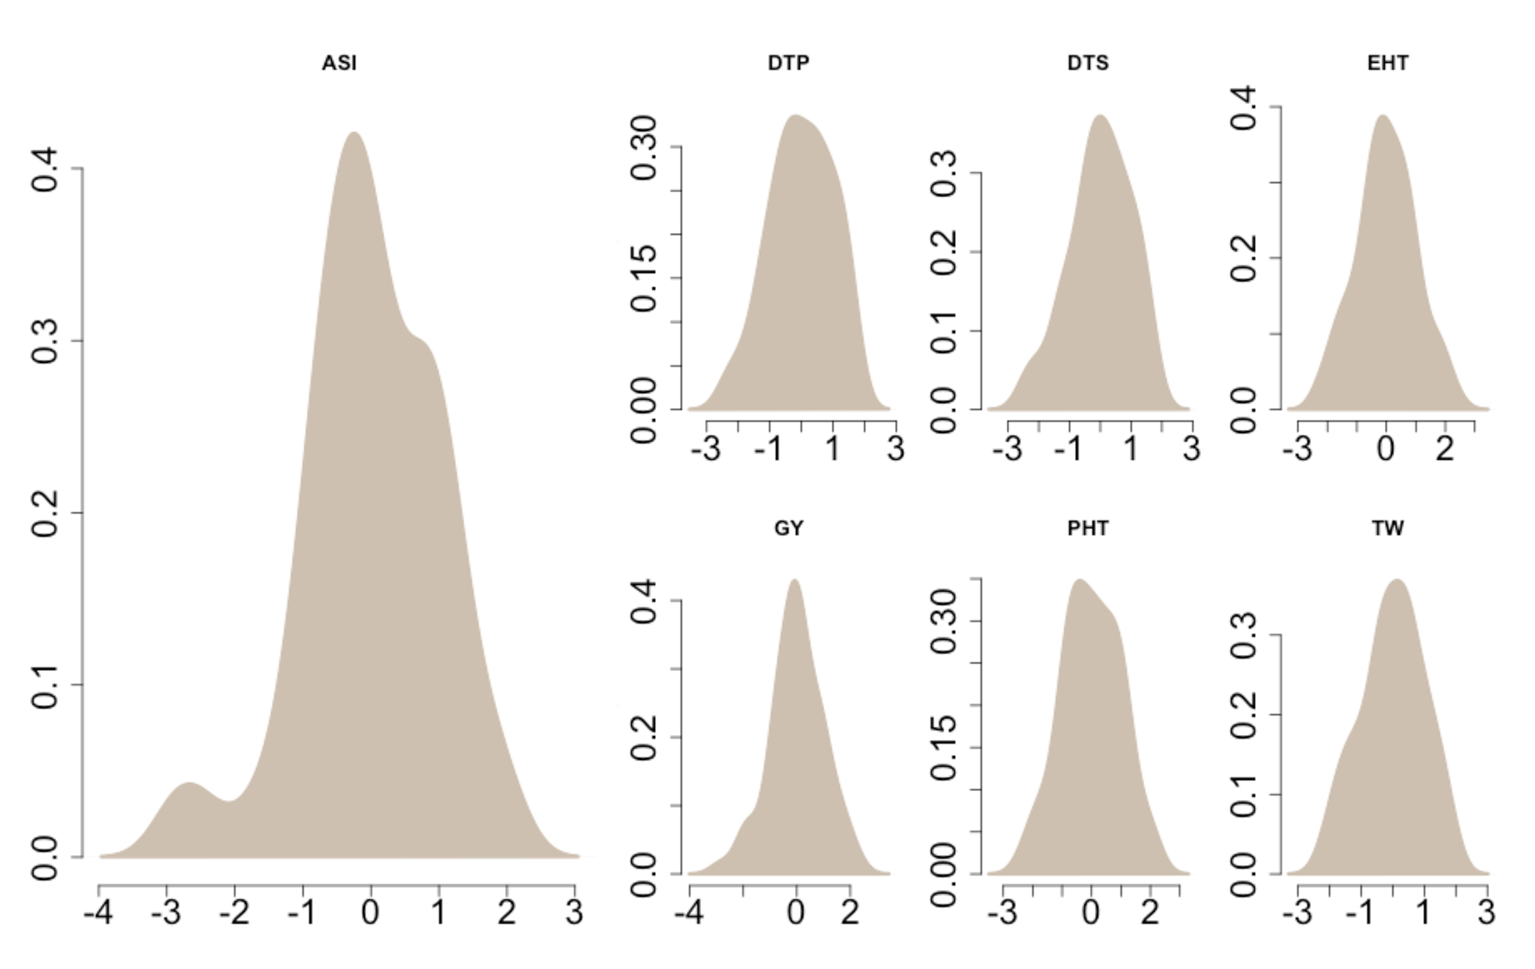
\includegraphics[width=\linewidth]{Figure_pheno.pdf}
\caption{\DIFaddFL{Density plots of the BLUE values for the seven phenotypic traits. On the x-axis, the phenotypic values were normalized.}}
\label{fig:pheno}
\end{figure}



\DIFaddend \subsection*{\DIFdelbegin \DIFdel{Evolutionary }\DIFdelend \DIFaddbegin \DIFadd{Sequence variation and evolutionary }\DIFaddend constraint\DIFdelbegin \DIFdel{information for genomic variants}\DIFdelend }

All twelve inbreds were sequenced to an average depth of $\sim$10X, resulting in a filtered set of 13.8 million SNPs. 
We estimated the allelic error rate using three independent data sets: for all individuals using 41,292 overlapping SNPs on the maize SNP50 bead chip \citep{Heerwaarden2012}; for all individuals using 180,313 overlapping SNPs identified through genotyping by sequencing (GBS) \citep{Romay2013}; and for B73 and Mo17 using the 10,426,715 SNP from the HapMap2 project \citep{Chia2012}.  \DIFdelbegin \DIFdelend Compared to corresponding SNPs identified by previous studies, a concordance rate of 99.1\% was observed. \DIFaddbegin \jri{Sofiane: can we separate those numbers out by study? or just report for one study and mention that similar rates were seen in other studies? either way it would be nice to know what rate went with what data. also is concordance mean identical genotype? do we have minor allele rate (which is a bit more informative)? if not, skip it.} 
\DIFaddend 

More than 86 million bp of the genome were annotated as conserved, with GERP scores $>0$.
Nonetheless, 506,898 of these sites were found to segregate among the 12 inbred parents of our diallel (Figure \ref{fig:gerpmaf}A and \ref{fig:dis1m}).
The minor allele frequency of SNPs at conserved sites was negatively correlated with GERP score (Figure \ref{fig:gerpmaf}B; \emph{P} value < 0.05, \emph{r} = $-0.8$), consistent with the idea that variants at sites with more positive GERP scores are more deleterious and more strongly impacted by purifying selection.

\begin{figure}[htbp]
\centering
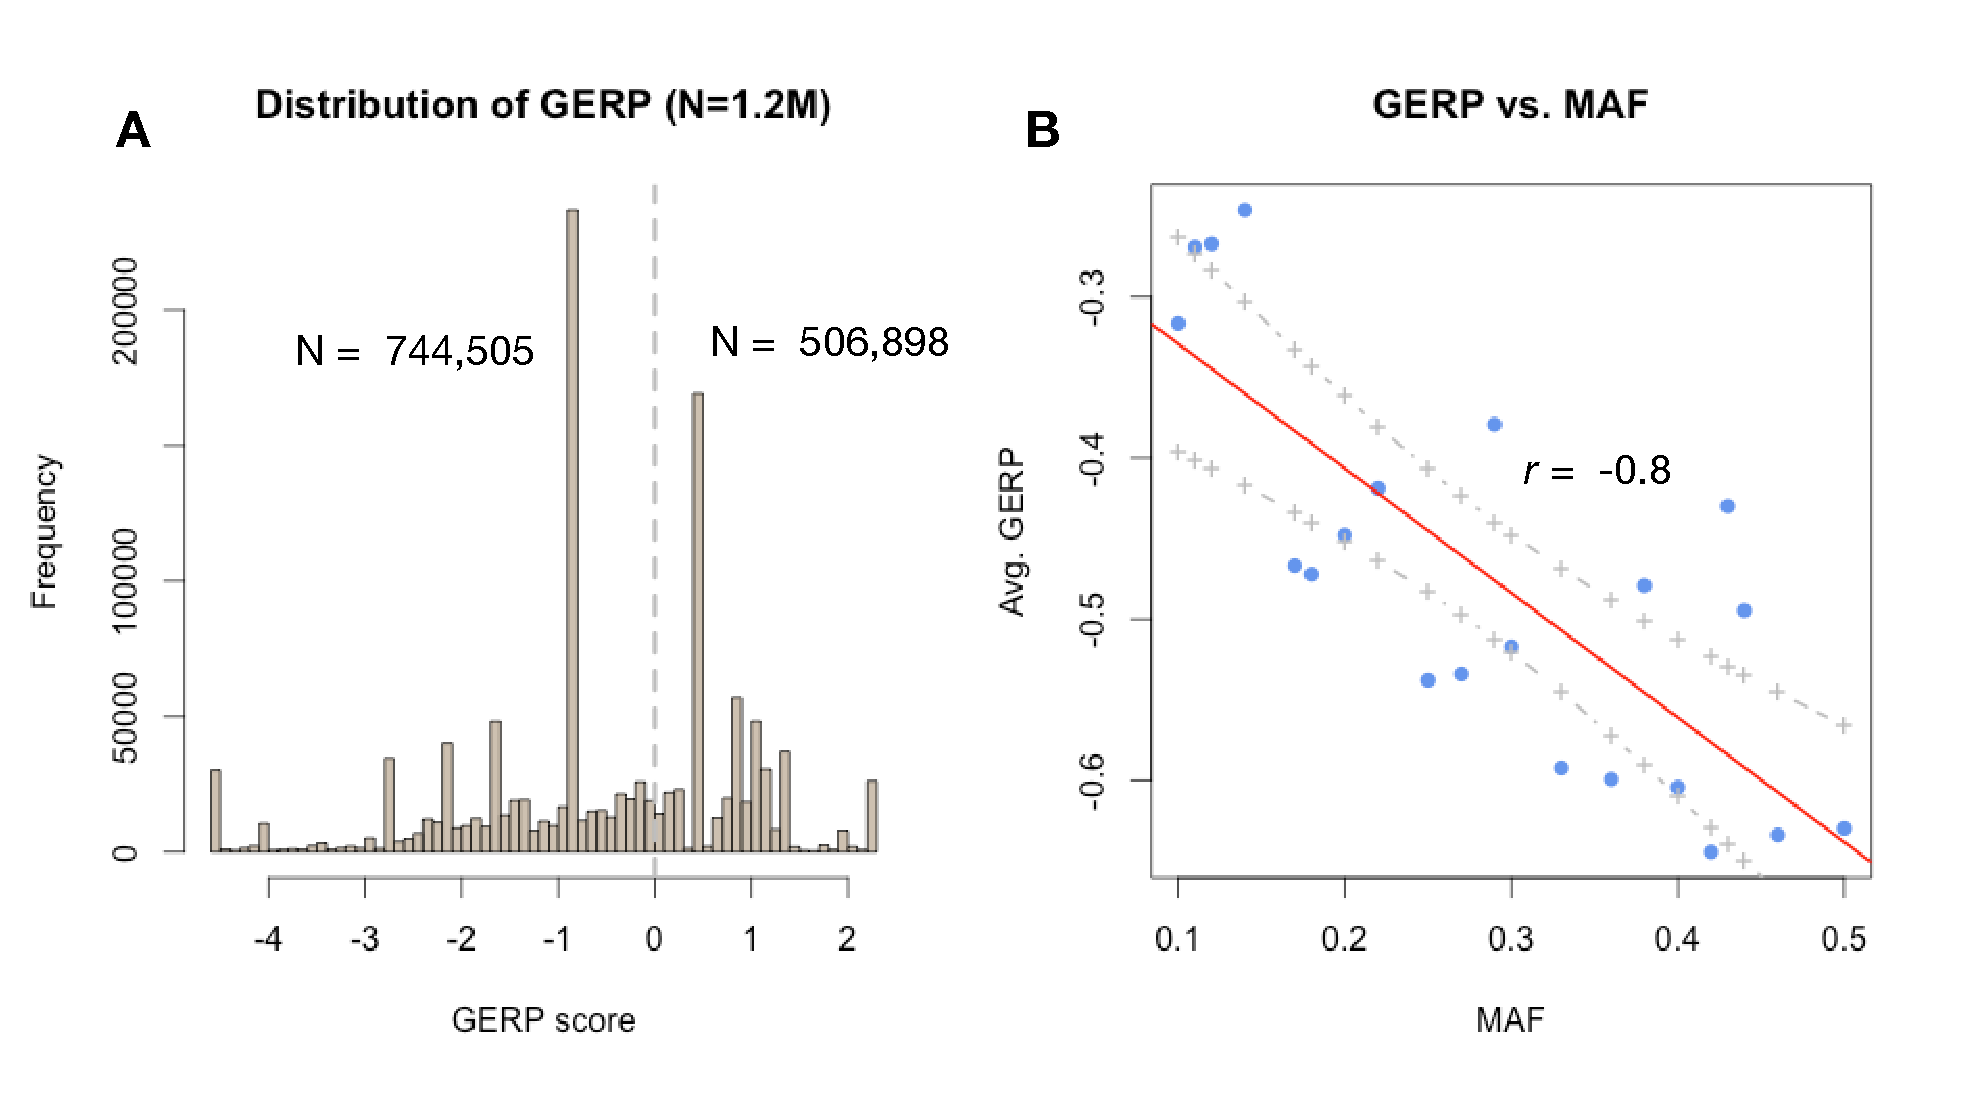
\includegraphics[width=\linewidth]{Figure_gerpmaf.pdf}
\caption{Distribution of GERP scores and relationship between GERP scores and MAFs. \textbf{(A)} Histogram of GERP scores \DIFdelbeginFL \DIFdelFL{extracted from }\DIFdelendFL \DIFaddbeginFL \DIFaddFL{at }\DIFaddendFL $\sim$\DIFdelbeginFL \DIFdelFL{1.2 }\DIFdelendFL \DIFaddbeginFL \DIFaddFL{1.3 }\DIFaddendFL million \DIFdelbeginFL \DIFdelFL{sites where the GERP scores were available}\DIFdelendFL \DIFaddbeginFL \DIFaddFL{SNPs}\DIFaddendFL . \DIFdelbeginFL \DIFdelendFL \textbf{(B)} Plot of average GERP scores in bins (bin size = 0.01) of minor allele frequency (MAF). \DIFdelbeginFL \DIFdelFL{The red }\DIFdelendFL \DIFaddbeginFL \DIFaddFL{Red }\DIFaddendFL and grey lines define the regression and its 95\% confidence interval.}
\label{fig:gerpmaf}
\end{figure}


\subsection*{\DIFdelbegin \DIFdel{Incorporatipn of GERP information improved }\DIFdelend \DIFaddbegin \DIFadd{Phenotypic }\DIFaddend prediction\DIFdelbegin \DIFdel{accuracies}\DIFdelend }

\DIFdelbegin \DIFdel{Genomic variants occurred at the evolutionary constraint sites were potentially deleterious. The phenotypic effects of these genetic loads and their contributions to heterosis become an interesting area to explore. However, the population size in this study is relative small and SNPs detected at sites containing high GERP scores are generally in low frequencies. The statistical power to detect the separate effects of these putative deleterious alleles becomes very low}\DIFdelend \DIFaddbegin \DIFadd{The small sample size of our diallel and the general low frequency of deleterious SNPs precludes association-based approaches to evaluate the impact of variants on phenotypic variation}\DIFaddend .
To alleviate \DIFdelbegin \DIFdel{the statistical limitations}\DIFdelend \DIFaddbegin \DIFadd{this limitation}\DIFaddend , we conceived a haplotype-based \DIFdelbegin \DIFdel{approach for GS, which could add up }\DIFdelend \DIFaddbegin \DIFadd{genomic selection approach in which we use estimates of evolutionary constraint across the genome \mbox{\citep{rodgers2015recombination}
}to sum the }\DIFaddend individual effects of deleterious alleles \DIFdelbegin \DIFdel{in IBD blocks and estimate these IBD blocks simultaneously. To conduct the analysis, first of all, 55,000 IBD blocks were identified, which had an average size of 44,980 bp (ranged from 36 to 10,320,000 bp). IBD blocks having > 1-kb in size and containing > 1 deleterious alleles (SNPs at sites with GERP scores >0) were kept for further analysis. Secondly, the GERP scores of SNPs in an IBD block were summed under both }\DIFdelend \DIFaddbegin \DIFadd{within IBD blocks under both an }\DIFaddend additive and dominant \DIFdelbegin \DIFdel{models. Those summed GERP scores on IBD blocks were considered as the measurements of the conservation of the haplotypes. More details of this procedure were illustrated in Figure \ref{fig:gerpibd}}\DIFdelend \DIFaddbegin \DIFadd{model (see Methods and Figure \ref{fig:gerpibd})}\DIFaddend . 

A Bayesian-based statistical method (BayesC) \citep{habier2011extension} \DIFaddbegin \DIFadd{using a 5-fold cross-validation approachwas }\DIFaddend was employed for model training. 
\DIFdelbegin \DIFdel{Using a 5-fold cross-validation approach, the prediction accuracies of the real data and cicularly shuffled data were compared. As shown in Figure \ref{fig:gerpall}, }\DIFdelend \DIFaddbegin \DIFadd{In general, average prediction accuracies were higher using the additive model (mean }\emph{\DIFadd{r}} \DIFadd{= 0.81 and 0.49 }\DIFaddend for traits \emph{per se} \DIFdelbegin \DIFdel{, prediction accuracies were significantly (FDR < 0.05)improved }\DIFdelend \DIFaddbegin \DIFadd{and BPH) than the dominant model (mean }\emph{\DIFadd{r}} \DIFadd{= 0.70 and 0.42), and accuracies for heterosis traits were lower than for traits }\emph{\DIFadd{per se}} \DIFadd{(Table \ref{table:table_s3}). }\jri{is there a table we can cite that has all these?} \yang{see edits}
\DIFadd{Incorporating evolutionary constraint information improved prediction accuracy }\DIFaddend for ASI and PHT \DIFdelbegin \DIFdel{when incorporating GERP information in the IBD blocks under the additive model ; prediction accuracy was significantly improved }\DIFdelend \DIFaddbegin \emph{\DIFadd{per se}} \DIFadd{under an additive model and }\DIFaddend for ASI under \DIFdelbegin \DIFdel{the dominant model . For heterosis transformation traits (BPH), incorporation of GERP scores improved BPH of }\DIFdelend \DIFaddbegin \DIFadd{a dominant model (FDR < 0.05, Figure \ref{fig:gerpall} A and B).
GERP scores also improved prediction accuracies of heterosis (BPH) for }\DIFaddend GY under the additive model and \DIFdelbegin \DIFdel{improved BPH of }\DIFdelend DTP, DTS and TW under the dominant model (\DIFaddbegin \DIFadd{FDR < 0.05, }\DIFaddend Figure \ref{fig:gerpall} C and D\DIFdelbegin \DIFdel{, Supplementary table 3). In general, the average prediction accuracis were higher using the additive model (mean }\emph{\DIFdel{r}} \DIFdel{= 0.81 and 0.49 for traits }\emph{\DIFdel{per se}} \DIFdel{and BPH) than the dominant model (mean }\emph{\DIFdel{r}} \DIFdel{= 0.70 and 0.42). And the prediction accuracies decreased for predicting heterosis transformations (BPH) as compared to the predictions for traits }\emph{\DIFdel{per se}}\DIFdelend \DIFaddbegin \DIFadd{)}\DIFaddend . \DIFdelbegin 
\DIFdel{It was argued that SNPs in genic regions might have higher GERP scores than those in non-genic regions. The circular shuffling permutations may shift the }\DIFdelend \DIFaddbegin \jri{ref/link to supp table 3 please. also, do we need to include FDR here? what are the multiple tests the FDR is correcting for here?} \yang{move table S3 to above. added FDR. FDR is for correcting multiple traits and multiple transformations.}
\DIFadd{To rule out the possible confounding of }\DIFaddend high GERP scores \DIFdelbegin \DIFdel{to non-genic regions. If that is the case, the approach tended to weigh more on genic SNPs. To rule out this possibility, we elected SNPs with GERP scores >0 in genic regions only and did the circular shuffling to assign GERP scores to the same set of the selected SNPs.  
By doing this , the method will not take advantage of genomic positional information any more. Noted that in this study less number of SNPs was selected (N = }\DIFdelend \DIFaddbegin \DIFadd{and genic annotations, we re-permuted the data using only deleterious (GERP $> 0$) genic SNPs.  
Though this resulted in fewer SNPs (}\DIFaddend 316, 983)\DIFdelbegin \DIFdel{. Nevertheless, }\DIFdelend \DIFaddbegin \DIFadd{, the }\DIFaddend model prediction accuracies \DIFdelbegin \DIFdel{were }\DIFdelend \DIFaddbegin \DIFadd{remained }\DIFaddend significantly improved for \DIFdelbegin \DIFdel{traits }\DIFdelend \DIFaddbegin \DIFadd{GY }\DIFaddend \emph{per se} \DIFdelbegin \DIFdel{of GY }\DIFdelend under the additive model \DIFdelbegin \DIFdel{. For heterosis transformations, prediction accuracies were significantly improved }\DIFdelend \DIFaddbegin \DIFadd{and }\DIFaddend for BPH of GY and PHT under the additive model \DIFdelbegin \DIFdel{and the prediction accuracy was significantly improved for pBPH of GY }\DIFdelend (Figure \ref{fig:genicsnp} and Table \DIFdelbegin \DIFdel{S4}\DIFdelend \DIFaddbegin \DIFadd{\ref{table:table_s4}}\DIFaddend ).   

\DIFaddbegin 


\DIFaddend \begin{figure}[htbp]
\centering
\DIFdelbeginFL \DIFdelendFL \DIFaddbeginFL 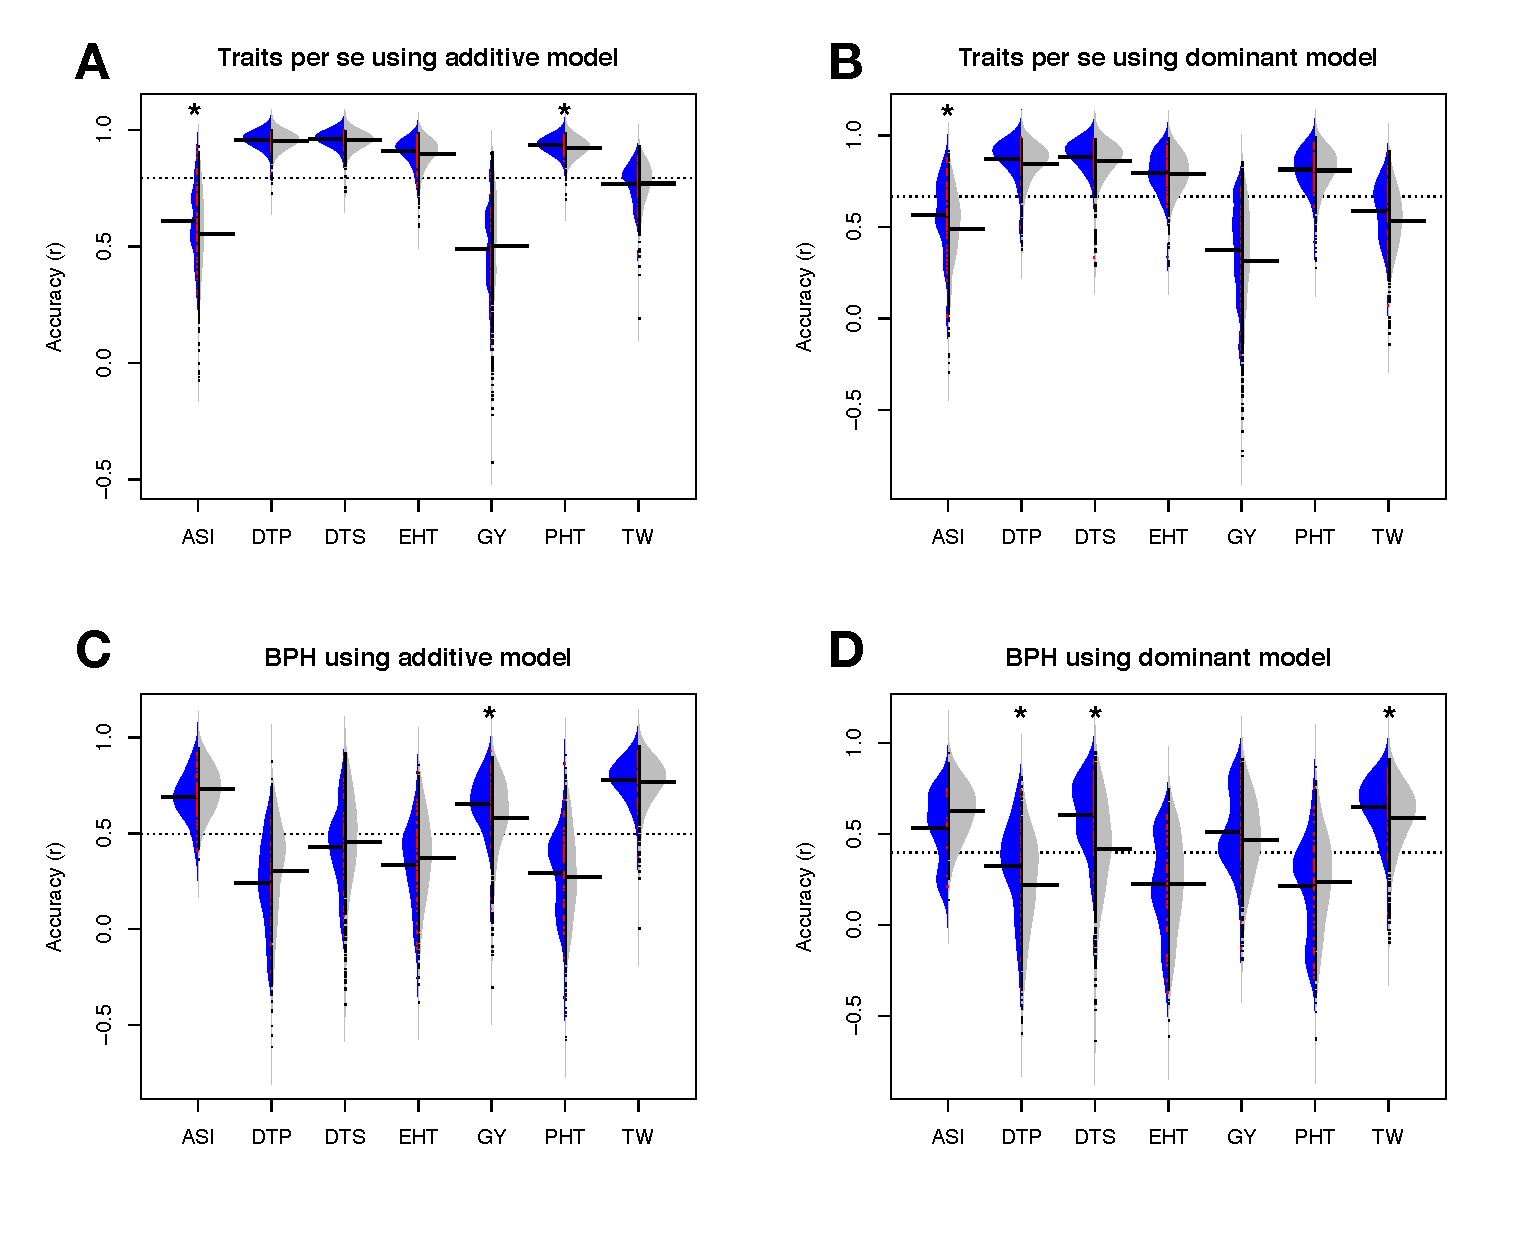
\includegraphics[width=\linewidth]{Figure_gerpall_m.pdf}
\DIFaddendFL \caption{Beanplots of cross-validation accuracies using SNPs with positive GERP \DIFdelbeginFL \DIFdelFL{score}\DIFdelendFL \DIFaddbeginFL \DIFaddFL{scores}\DIFaddendFL . Cross-validation experiments were conducted using selected SNPs and \DIFdelbeginFL \DIFdelFL{circular shuffled }\DIFdelendFL \DIFaddbeginFL \DIFaddFL{permuted }\DIFaddendFL data \DIFdelbeginFL \DIFdelFL{from the same set of SNPs }\DIFdelendFL for traits \emph{per se} (\textbf{A, B}) \DIFdelbeginFL \DIFdelFL{, }\DIFdelendFL \DIFaddbeginFL \DIFaddFL{and }\DIFaddendFL BPH (\textbf{C, D}) \DIFdelbeginFL \DIFdelFL{and pBPH (}\textbf{\DIFdelFL{E, F}}\DIFdelFL{) }\DIFdelendFL under additive (\DIFdelbeginFL \textbf{\DIFdelFL{A, C, E}}\DIFdelendFL \DIFaddbeginFL \textbf{\DIFaddFL{A and C}}\DIFaddendFL ) and dominant (\DIFdelbeginFL \textbf{\DIFdelFL{B, D, F}}\DIFdelendFL \DIFaddbeginFL \textbf{\DIFaddFL{B and D}}\DIFaddendFL ) models. Accuraries from the real data were plotted on the left \DIFdelbeginFL \DIFdelFL{side of the bean }\DIFdelendFL (blue) and permutation results \DIFdelbeginFL \DIFdelFL{plotted }\DIFdelendFL on the right (grey). Horizotal bars \DIFdelbeginFL \DIFdelFL{on beans }\DIFdelendFL indicate mean accuracies \DIFdelbeginFL \DIFdelFL{. The }\DIFdelendFL \DIFaddbeginFL \DIFaddFL{for each trait and the }\DIFaddendFL grey dashed lines indicate the overall \DIFdelbeginFL \DIFdelFL{average accuracies}\DIFdelendFL \DIFaddbeginFL \DIFaddFL{mean accuracy}\DIFaddendFL . Stars indicate significantly \DIFdelbeginFL \DIFdelFL{improved cross-validation accuracies with }\DIFdelendFL \DIFaddbeginFL \DIFaddFL{(}\DIFaddendFL FDR < 0.05\DIFaddbeginFL \DIFaddFL{) higher cross-validation accuracies}\DIFaddendFL .  }
\label{fig:gerpall}
\end{figure}

\subsection*{Posterior phenotypic variance explained and model comparisons}

To learn why the prediction performace varied among traits \emph{per se} and heterosis\DIFdelbegin \DIFdel{transformations}\DIFdelend , we obtained the posterior variance explained by our models using the complete set of data. 
As shown in Figure \ref{fig:h2}, additive models explained more phenotypic variance for traits \emph{per se} of DTP, DTS, EHT and PHT; but explained less phenotypic variance for heterosis \DIFdelbegin \DIFdel{transformations }\DIFdelend (BPH) of ASI, GY and TW. 
\DIFdelbegin \DIFdel{On the contrary, lager proportions }\DIFdelend \DIFaddbegin \DIFadd{In contrast, a larger proportion }\DIFaddend of the phenotypic variance could be explained by the dominant models for heterosis \DIFdelbegin \DIFdel{transformations }\DIFdelend (BPH) of ASI, GY and TW. 
\DIFdelbegin \DIFdel{For the GY in particular, 50}\DIFdelend \DIFaddbegin \DIFadd{This difference was particularly striking for grain yield under the dominant model, where only 3}\DIFaddend \% of the \DIFdelbegin \DIFdel{heterosis }\DIFdelend \DIFaddbegin \DIFadd{variance in trait }\emph{\DIFadd{per se}} \DIFaddend could be explained \DIFdelbegin \DIFdel{by dominant model}\DIFdelend \DIFaddbegin \DIFadd{but 61\% of the variance in BPH was explained}\DIFaddend . 

Heterosis transformations were largely determined by the accuracies of the parental phenotypes. 
To take the uncertainty of the parental phenotypes into consideration, we estimated  \DIFdelbegin \DIFdel{the combining abilities }\DIFdelend \DIFaddbegin \DIFadd{combining ability }\DIFaddend from the hybrid population itself to investigate which modes of inheritance perform better than the null models. 
We extracted the breeding values estimated \DIFdelbegin \DIFdel{with }\DIFdelend \DIFaddbegin \DIFadd{under }\DIFaddend both additive and dominant models using \DIFdelbegin \DIFdel{the genome-wide IBD blocks incorporated with the }\DIFdelend \DIFaddbegin \DIFadd{our haplotype blocks and incorporating }\DIFaddend GERP scores. 
\DIFdelbegin \DIFdel{Consistent with above analysis, IBD blocks coded with dominant mode of inheritance significantly (equation \ref{eq:refname1} vs. equation \ref{eq:refname2}, ANOVA }\emph{\DIFdel{P}} \DIFdel{value < 0.05 ) improved model fitting for ASI and GY. We also compared model \ref{eq:refname3} and model \ref{eq:refname4}, ANOVA results indicated that \ref{eq:refname4} performed almost as good as \ref{eq:refname3}, indicating that specific combining ability captured most of the parental interactions and the current method could not detect higher order of interactions. 
}
\DIFdelend \DIFaddbegin \DIFadd{We then applied the following models:
}\DIFaddend \begin{equation}
Y_{ij} = \mu + GCA_{i} + GCA_{j} + \varepsilon
\label{eq:refname1}
\end{equation}
\begin{equation}
Y_{ij} = \mu + GCA_{i} + GCA_{j} +  G_{ij} + \varepsilon
\label{eq:refname2}
\end{equation}
\begin{equation}
Y_{ij} = \mu + GCA_{i} + GCA_{j} + SCA_{ij} + \varepsilon
\label{eq:refname3}
\end{equation}
\begin{equation}
Y_{ij} = \mu + GCA_{i} + GCA_{j} + SCA_{ij} + G_{ij} + \varepsilon
\label{eq:refname4}
\end{equation}
where 
$Y_{ij}$ is the BLUE value of the hybrid crossed between the $i^{th}$ inbred and $j^{th}$ inbred; 
$\mu$, the overall mean; 
$GCA_{i}$, the general combining ability of the $i^{th}$ inbred;
$GCA_{j}$, the general combining ability of the $j^{th}$ inbred;
$SCA_{ij}$, the specific combining ability of between the $i^{th}$ and $j^{th}$ inbreds;
\DIFaddbegin \DIFadd{$G_{ij}$, breeding values estimated by our GS model for hybrid crossed between the $i^{th}$ inbred and $j^{th}$ inbred; 
}\DIFaddend $\varepsilon$, the model residuals.

\DIFaddbegin \DIFadd{Consistent with the previous analysis, haplotype blocks coded with the dominant mode of inheritance significantly  improved model fitting for ASI and GY (equation \ref{eq:refname1} vs. equation \ref{eq:refname2}, ANOVA }\emph{\DIFadd{P}} \DIFadd{value $<0.05$, Table \ref{table:table_s5}). 
Comparison of model \ref{eq:refname3} and model \ref{eq:refname4} indicated that model \ref{eq:refname4} performed almost as well as \ref{eq:refname3} (ANOVA }\emph{\DIFadd{P}} \DIFadd{value = }\X\DIFadd{), indicating that specific combining ability captured most of the parental interactions and the current method could not detect higher order of interactions. }\jri{does model 2 outperform model 1? does 3 outperform 2? 4 should outperform 3 because it has extra parameters, but the text says ``almost as well''?}
\yang{We are comparing [1 and 2], [3 and 4] only by adding breeding value estimated from our GERP GS model. I do not think this result add anything to our story. maybe we will ditch it?}


\DIFaddend \begin{figure}[htbp]
\centering
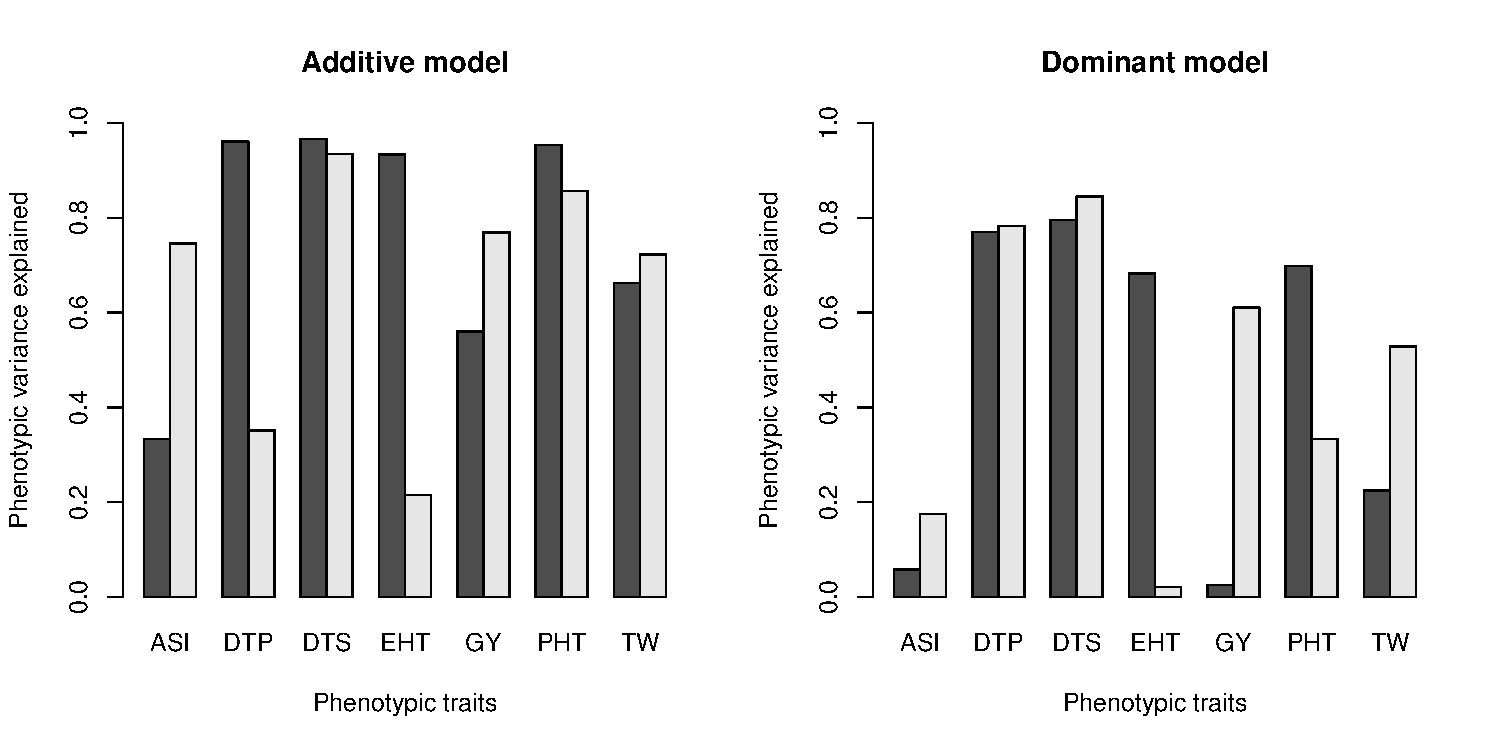
\includegraphics[width=\linewidth]{Figure_h2.pdf}
\caption{\DIFdelbeginFL \DIFdelFL{Barplots of the }\DIFdelendFL \DIFaddbeginFL \DIFaddFL{Posterior }\DIFaddendFL phenotypic variance explained by \DIFaddbeginFL \DIFaddFL{deleterious genic SNPs in }\DIFaddendFL IBD blocks \DIFdelbeginFL \DIFdelFL{incorporated with GERP scores}\DIFdelendFL \DIFaddbeginFL \DIFaddFL{using additive and dominant models}\DIFaddendFL . \DIFaddbeginFL \DIFaddFL{Dark color indicates trait }\emph{\DIFaddFL{per se}} \DIFaddFL{and grey color indicates BPH. }\DIFaddendFL }  
\label{fig:h2}
\end{figure}


\section*{Discussion}

\begin{itemize}
  \item do we support deleterious model of Mezmouk et al.? \yang{yes}
  \item how do results match with heritability and heterosis? \yang{and mode of inheritance}
  \item Indication for breeding? genomic selection using GERP and other annotation information. 
\end{itemize}


In this study \DIFdelbegin \DIFdel{, }\DIFdelend \DIFaddbegin \DIFadd{we have identified }\DIFaddend more than 500,000 deleterious SNPs \DIFdelbegin \DIFdel{were identified in }\DIFdelend \DIFaddbegin \DIFadd{in panel of }\DIFaddend elite maize lines.
On average, each elite inbred line carries about 100,000 deleterious SNPs (GERP > 0). \DIFdelbegin \DIFdel{In the population}\DIFdelend \DIFaddbegin \jri{cool, this should be mentioned here but also in the results. is there any big variation?  some lines more than others? is mo17 worse than the pvps? given the comment below i added about linkage, can we calculate mean deleterious variants per cM?  that would be sweet to know and to point out that there are tons around the centromere}
\DIFadd{Across lines}\DIFaddend , however, \DIFaddbegin \DIFadd{the }\DIFaddend majority of these deleterious mutations were maintained \DIFdelbegin \DIFdel{in a }\DIFdelend \DIFaddbegin \DIFadd{at }\DIFaddend low frequency, \DIFdelbegin \DIFdel{which }\DIFdelend consistent with previous \DIFdelbegin \DIFdel{observation }\DIFdelend \DIFaddbegin \DIFadd{observations }\DIFaddend \citep{rodgers2015recombination}. 
The large number of \DIFdelbegin \DIFdel{deleterious alleles }\DIFdelend \DIFaddbegin \DIFadd{linked deleterious alleles present would likely }\DIFaddend make it hard to \DIFdelbegin \DIFdel{be completely purged }\DIFdelend \DIFaddbegin \DIFadd{completely purge all such alleles }\DIFaddend through breeding efforts. \DIFdelbegin \DIFdel{In practice, part of the genetic loads could be released in F1 hybrids by combining appropriate inbred lines (from pre-defined heterotic groups) to complement deleterious alleles}\DIFdelend \DIFaddbegin \DIFadd{Instead, breeders have devised a strategy --- hybrid breeding --- that may circumvent much of this problem via complementation}\DIFaddend .
Indeed, results in this study \DIFdelbegin \DIFdel{shown }\DIFdelend \DIFaddbegin \DIFadd{show }\DIFaddend that prediction accuracies were higher for yield heterosis \DIFdelbegin \DIFdel{using deleterious SNPs than permuted ones.  
Because we weighted SNPs with their conservation score in GS model, the improved accuracies could be attributed to deleteriousness of SNP variants.
Therefore, it provided evidence of complementation of deleterious alleles for heterosis \mbox{\citex{}
}. 
Note that thousands of deleterious alleles may be involved in the }\DIFdelend \DIFaddbegin \DIFadd{when information about deleterious SNPs was incorporated into the prediction model.  
Because there are likely  thousands of deleterious alleles involved in }\DIFaddend complementation, \DIFdelbegin \DIFdel{and most of which may have minor effects. 
Their effects could not be easily detected by traditional QTL or GWAS \mbox{\citex{}
}. 
}\DIFdelend \DIFaddbegin \DIFadd{many with relatively small effects, traditional GWAS approaches with genome-wide thresholds of multiple testing are likely unable to detect such effects.
Using a liberal significance threshold, however, our previous efforts nonetheless showed an enrichment for deleterious genic SNPs among associated markers for a number of traits \mbox{\citep{Mezmouk2014}
}.
}\DIFaddend 

\DIFdelbegin \DIFdel{To test }\DIFdelend \DIFaddbegin \DIFadd{Our models did not increase the prediction accuracies equally well for traits }\emph{\DIFadd{per se}} \DIFadd{and their heterosis transformations. 
This is not surprising, however, given that the variation in genetic architectures of different phenotypic traits --- flowering time, for example, appears primarily determined by many loci of small additive effect \mbox{\citep{buckler2009genetic}
}, while }\X \jri{better to use another maize example if we can rather than rice...}\DIFadd{. 
Consistent with this, we observed that the additive model increased prediction accuracies for ASI as a trait }\emph{\DIFadd{per se}} \DIFadd{and }\jri{ideally above use a phenotype we can compare in this way... dominant model increased the prediction accuacies for trait \emph{per se} of GY.} 
\DIFadd{One limitation of our current models is that we assume phenotypic traits are determined by complete additive or complete dominant effects. 
Traits with a mixture of additive and dominant casual loci may thus fail to be predicted. 
Another limitaiton is likely the population size used; we may simply not have enough power to predict traits with low heritability. 
}


\DIFadd{To test the simple complementation }\DIFaddend hypothesis, we developed a GS pipeline, which incorporated evolutionary conservation information in the GS model. As the genotyping cost keeps declining, GS \DIFdelbegin \DIFdel{tends to replace marker assistant selection (MAS) \mbox{\citex{}
}}\DIFdelend \DIFaddbegin \DIFadd{gains its popularity }\DIFaddend in plant breeding \DIFdelbegin \DIFdel{\mbox{\citex{}
}. Researchers developed a series of }\DIFdelend \DIFaddbegin \DIFadd{\mbox{\citep{desta2014genomic}
}. Previous studies mainly focused on developing }\DIFaddend statistical approaches to improve the efficiency of GS model\DIFdelbegin \DIFdel{\mbox{\citex{}
}}\DIFdelend , however, none of the existing \DIFdelbegin \DIFdel{approaches }\DIFdelend \DIFaddbegin \DIFadd{studies }\DIFaddend have taken prior biological information into consideration. It is known that SNP variations would have varied impacts depending on their genomic position (e.g. ) \citex{}, biological function (e.g. transcription binding sites) and evolutionary conservation. The incorporation of GERP information under the Bayesian framework developed in this study is the first step towarding more meaningful models for further GS.     

\DIFdelbegin \DIFdel{It was not surprised that the current models did not increase the prediction accuacies equally well for traits }\emph{\DIFdel{per se}} \DIFdel{and their heterosis transformations. Genetic arachitectures of different phenotypic traits varied in maize and other crop species, e.g., flowering time of maize was determined by many small effect additive loci \mbox{\citex{}
}and rice yield was determined by many dominant loci \mbox{\citex{}
}. Weobserved additive model increased the prediction accuacies for trait }\emph{\DIFdel{per se}} \DIFdel{of ASI and dominant model increased the prediction accuacies for trait }\emph{\DIFdel{per se}} \DIFdel{of GY. Because under current models, we simply assume phenotypic traits were determined by complete additive or complete dominant effects. Traits with mixture effects of additive and dominant loci may fail to be predicted. In addition, the population size was relative small in the model training, we may not have enough power to predict traits with low heritability. 
}
\DIFdelend 

\DIFaddbegin \section*{\DIFadd{Acknowledgements}}
\DIFadd{Financial support for this work came from NSF (grants IOS-0820619 and IOS-1238014), USDA (grants 2009-65300-05668 and }\X\DIFadd{), DuPont Pioneer, and N2 Genetics. We'd like to thank Graham Coop, James Holland, }\X\DIFadd{, and }\X \DIFadd{reviewers for helpful discussion. 
}

\DIFaddend 
\clearpage
\bibliography{Diallel}



\onecolumn
\pagebreak
\beginsupplement

\section*{Supporting Information}

\DIFdelbegin \DIFdelend \DIFaddbegin \begin{table}[htbp]
\caption{\DIFaddFL{BLUE values of the seven phenotypic traits. (}\url{https://github.com/RILAB/pvpDiallel/blob/master/manuscript/Figure_Table/Table_S1.trait_matrix.csv}\DIFaddFL{)}}
\label{table:table_s1}
\end{table}
\DIFaddend 

\DIFdelbegin \textbf{\DIFdel{Diallel experimental design and distribution of phenotypic data.}}
\textbf{\DIFdel{(A)}} \DIFdel{Twelve maize inbred lines were selected and crossed in a partial diallel. }\textbf{\DIFdel{(B)}} \DIFdel{Density plots of the phenotypic distributions.
}\DIFdelend \DIFaddbegin \begin{table}[htbp]
\caption{\DIFaddFL{General combining ability and specific combining ability of the seven phenotypic traits. (}\url{https://github.com/RILAB/pvpDiallel/blob/master/manuscript/Figure_Table/Table_S2.CA.csv}\DIFaddFL{)}}
\label{table:table_s2}
\end{table}
\DIFaddend 

\DIFaddbegin \begin{table}[htbp]
\caption{\DIFaddFL{Cross-validation results using all genome-wide deleterious SNPs. (}\url{https://github.com/RILAB/pvpDiallel/blob/master/manuscript/Figure_Table/Table_S3_allsnps_FDR.csv}\DIFaddFL{)}}
\label{table:table_s3}
\end{table}

\begin{table}[htbp]
\caption{\DIFaddFL{Cross-validation results using deleterious genic SNPs. (}\url{https://github.com/RILAB/pvpDiallel/blob/master/manuscript/Figure_Table/Table_S4_genicsnps_FDR.csv}\DIFaddFL{)}}
\label{table:table_s4}
\end{table}

\begin{table}[htbp]
\caption{\DIFaddFL{ANOVA P values of model comparisons. (}\url{https://github.com/RILAB/pvpDiallel/blob/master/manuscript/Figure_Table/Table_S5_model_comp.csv}\DIFaddFL{)}}
\label{table:table_s5}
\end{table}

\DIFaddend \begin{figure}[htbp]
\centering
\DIFaddbeginFL 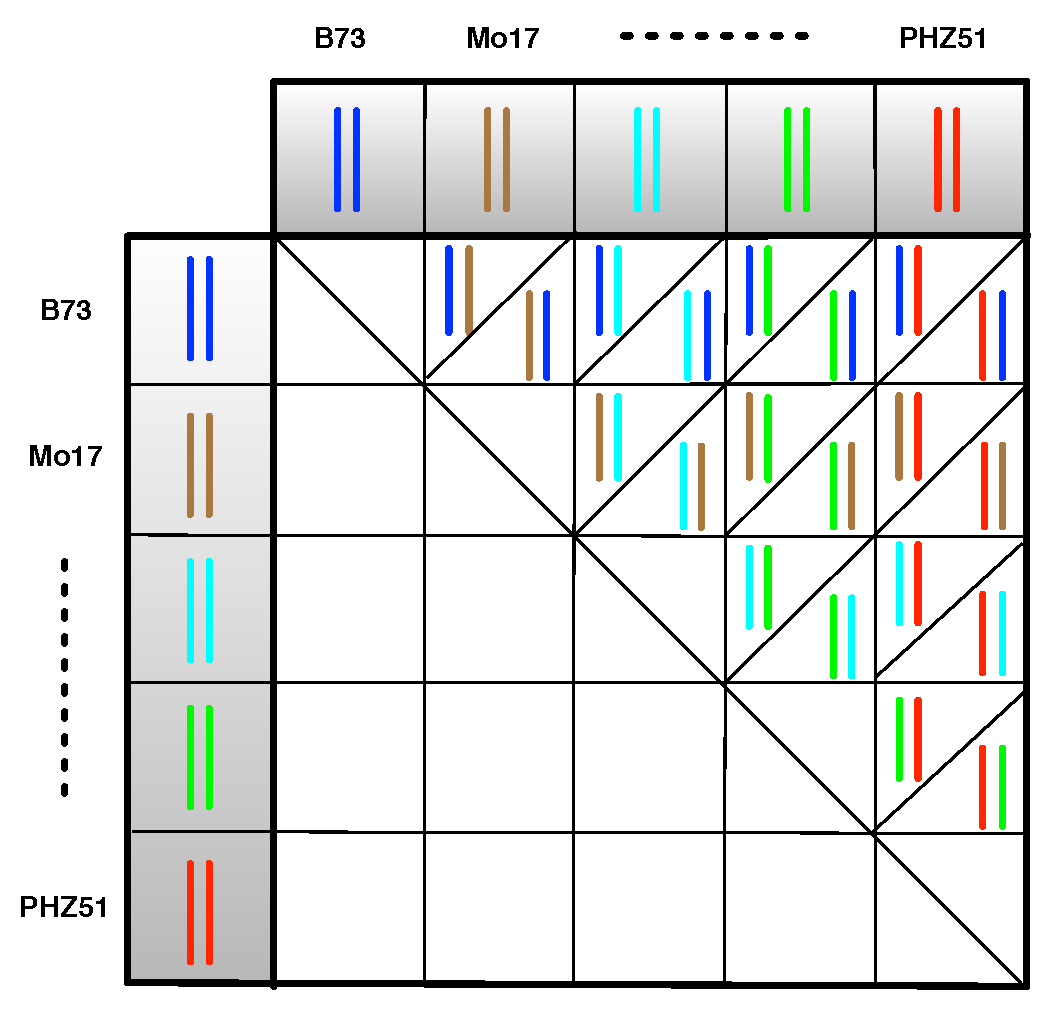
\includegraphics[width=\linewidth]{SFig_diallel.pdf}
\caption{\DIFaddFL{Twelve maize inbred lines were selected and crossed in a partial diallel fashion. Each inbred lines was used as both male and female and the resulting F1s were bulked. }\jri{do we need to modify this diagram now that we now reciprocal crosses were pooled?} \yang{any other idea to re-design the figure? or ditch it?} \jri{this isn't bad, but what deleting the bottom triangle completely rather than leave the cells blank?} }
\label{fig:diallel}
\end{figure}


\begin{figure}[htbp]
\centering
\DIFaddendFL 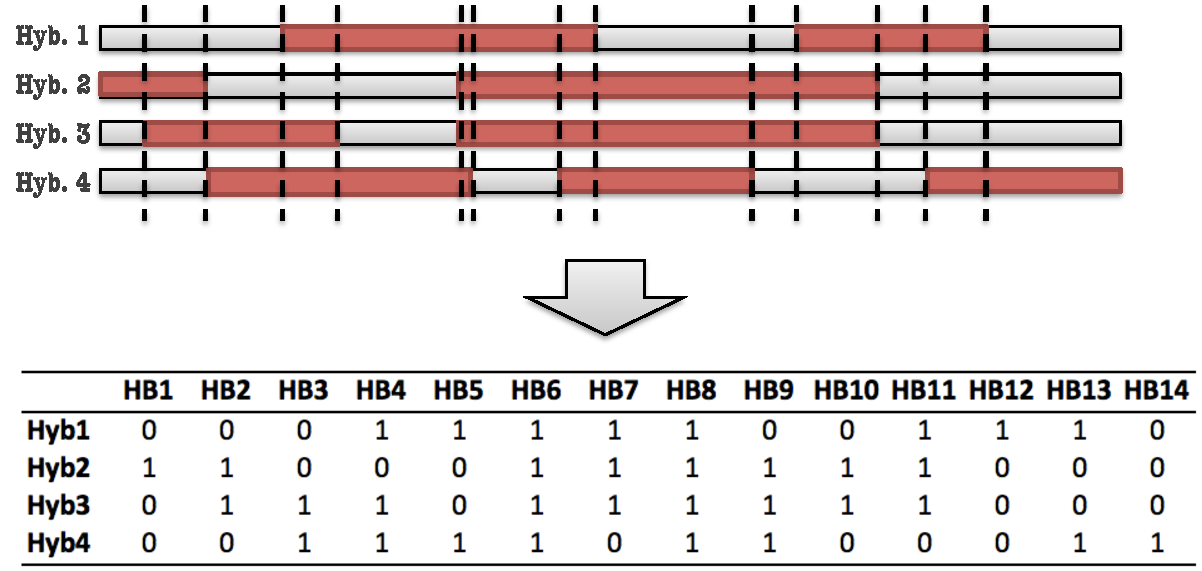
\includegraphics[width=\linewidth]{SFig_define_IBD.pdf}
\caption{Haplotype block identification using an IBD approach. In the upper panel, regions in red are IBD blocks identified by pairwise comparison of the two parental lines of a hybrid. The vertical dashed lines define haplotype blocks. In the lower panel, hybrid genotypes at each block are coded as heterozygotes (0) or homozygotes (1).}
\label{fig:defineibd}
\end{figure}



\begin{figure}[htbp]
\centering
\includegraphics[width=\linewidth]{SFig_pBPH.pdf}
\caption{Boxplot of percent best parent heterosis (pBPH). In the plot, ASI was calculated using pBPHmin and the other six traits were calculated using pBPHmax.}
\label{fig:pBPH}
\end{figure}

\begin{figure}[htbp]
\centering
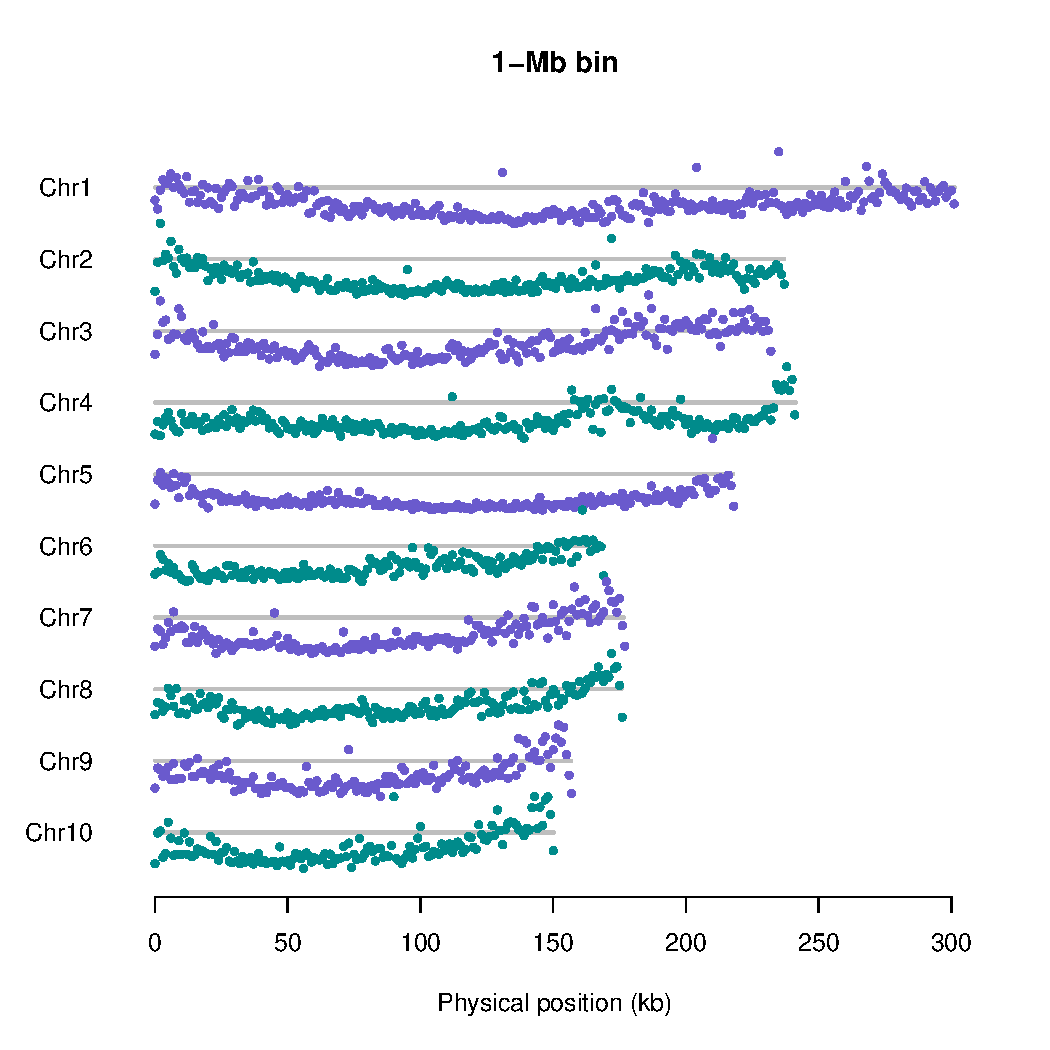
\includegraphics[width=\linewidth]{SFig_gerp_dis1m.pdf}
\caption{GERP score distribution across the genome. Shown are mean GERP scores in a 1-Mb bin region.}
\label{fig:dis1m}
\end{figure}

\DIFdelbegin \DIFdelend \DIFaddbegin \begin{figure}[htbp]
\DIFaddendFL 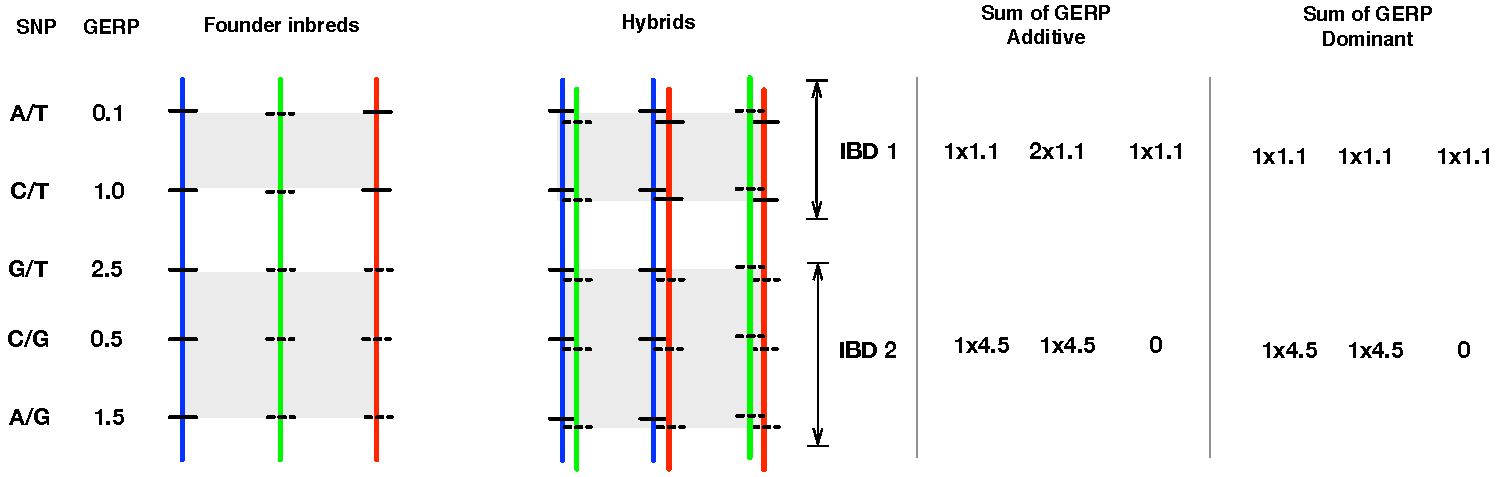
\includegraphics[width=0.9\textwidth]{SFig_gerpIBD.pdf}
\caption{
\textbf{Incoporation of conservation information into IBD blocks.}
Regions of the genome that are identical by descent (IBD) among the 12 inbreds were identified using Beagle \citep{Browning2009}.  The GERP scores of SNPs in an IBD block were summed under both additive and dominant models. For a particular SNP with GERP score $g$, the homozygous non-reference genotype was assigned a value of $2g$, the heterozygote assigned a value of $g$, and the reference homozygote a value of 0.  Under the dominant model, both the heterozygote and the non-reference homozygote were assigned a value of $g$, with the reference homozygote again assigned a value of 0.}
\label{fig:gerpibd}
\end{figure}

\begin{figure}[htbp]
\centering
\DIFdelbeginFL \DIFdelendFL \DIFaddbeginFL 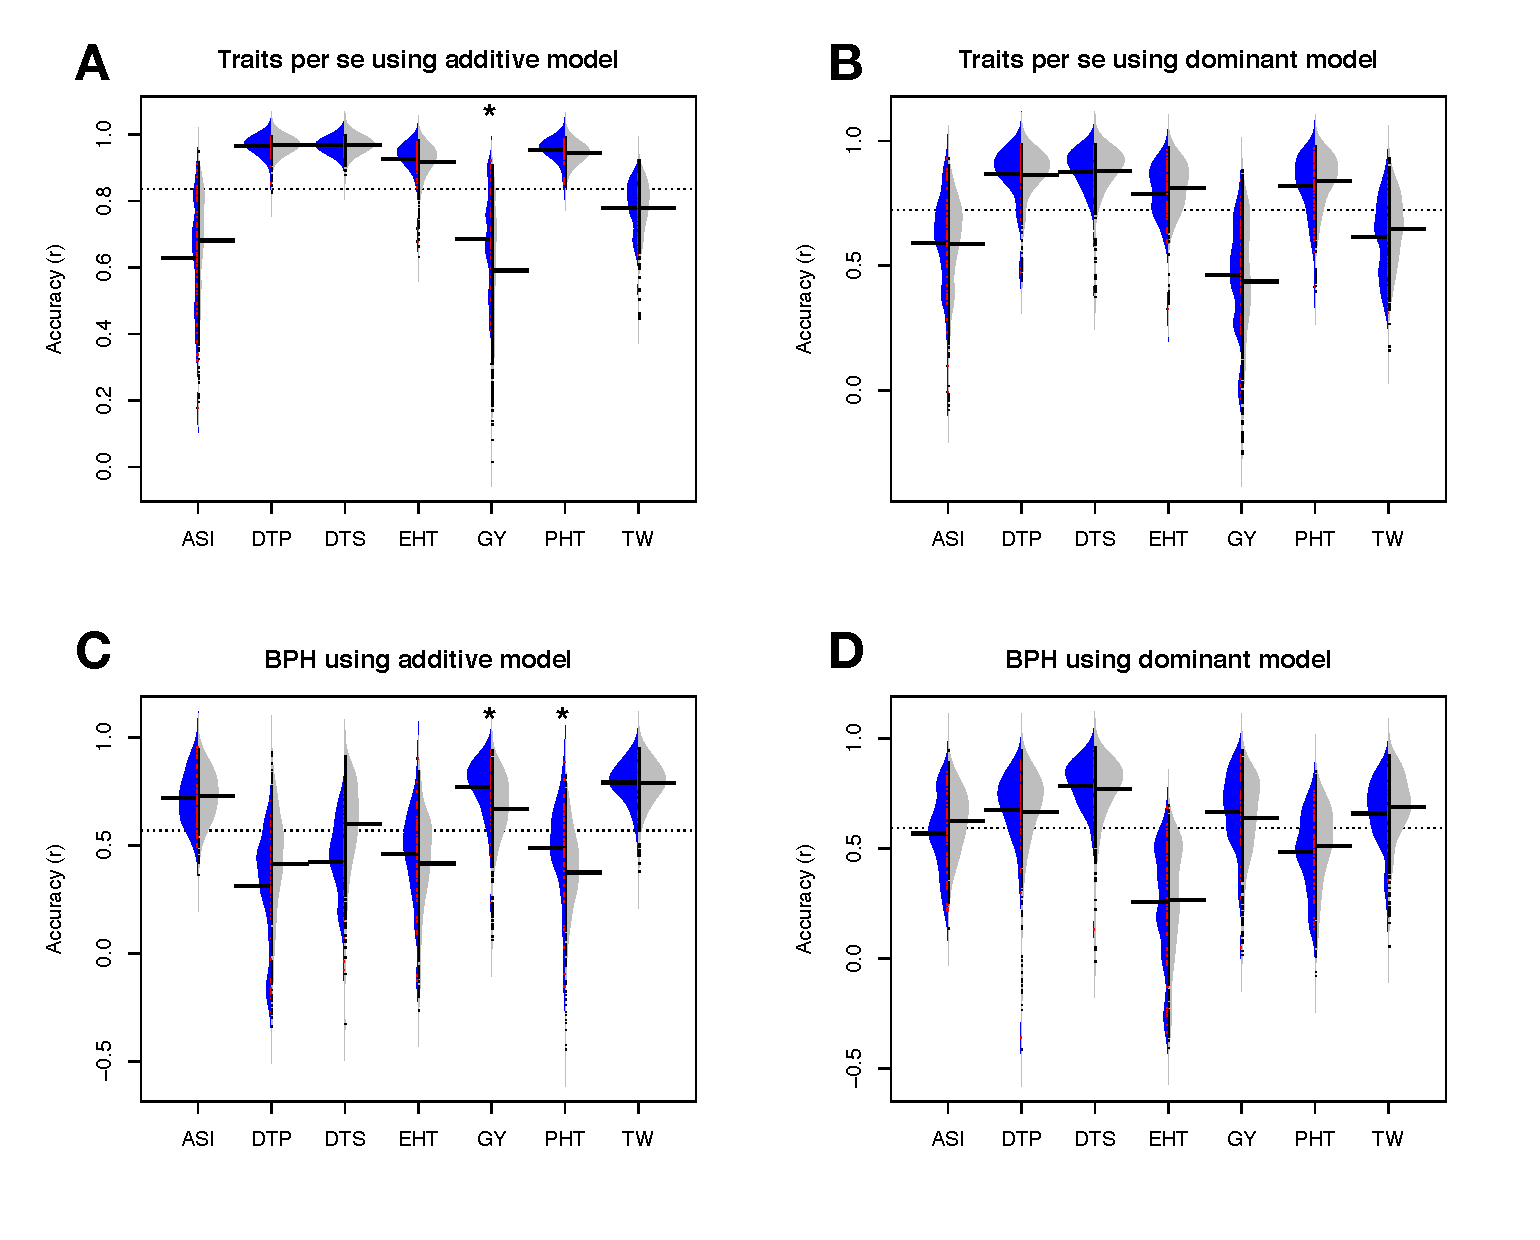
\includegraphics[width=\linewidth]{SFig_genicsnp_m.pdf}
\DIFaddendFL \caption{Cross-validation accuracies using genic SNPs. Cross-validation experiments were conducted using genic SNPs and compared to circular-shuffled data for traits \emph{per se} (\textbf{A, B}) and pBPH (\textbf{C, D}) under additive (\textbf{A, C}) and dominant (\textbf{B, D}) models. Distirbutions show accuracty of prediction from real data (blue) and permutations (grey), with horizontal bars to indicate mean accuracy.  Stars indicate significantly higher cross-validation accuracy for the real data.  The average accuracy across all traits is shown with the grey dotted line. }
\label{fig:genicsnp}
\end{figure}

\end{document}